\documentclass{article}

\usepackage{sectsty}
\usepackage{amssymb}
\usepackage{amsmath}
\usepackage{graphicx}
\usepackage{listings}

\begin{document}

% title stuff
\title{Interactive Fractal Viewer \\
CSEE W4840 Project Design}
\author{Nathan Hwang - nyh2105@columbia.edu \and
Richard Nwaobasi - rcn2105@columbia.edu \and
Stephen Pratt - sdp2128@columbia.edu \and
Luis Pe\~{n}a - lep2141@columbia.edu}
\maketitle
\newpage
\abstract{Fractals are often appreciated for their rich and elegant
  internal complexity. This complexity is responsible for the
  beautiful aesthetic of these famed mathematical images as well as
  the amount of computational power required to generate them. Using
  fixed point calculations within parallelized sequential logic
  blocks, we aim to develop an hardware-accelerated fractal generator,
  capable of computing and displaying quadratic Julia sets in
  significantly less time than a software-based solution.}

% ------------------------------------------------------------
% and we begin the design document proper



% ------------------------------------------------------------
\section{High-level Overview}

The following is a description the high-level block structure of the project:

\begin{itemize}
\item A Window Generator builds a set of 4-tuples $(x, y, a, b)$ where
  each tuple is a mapping from a VGA coordinate $(x, y)$ to a value in
  the complex plane of the form $a+bi$. The Window Generator is
  implemtented by the Nios II processor.
\item The processor writes its values across its bus into a queue,
  which feeds values to Iterative Function Modules (IFMs).
\item Each IFM computes the number of function iterations required for
  a specified value to become unbounded. Multiple IFMs work in
  parallel.
\item Another queue recieves 3-tuples $(x, y, c)$ from the IFMs, where
  $(x, y)$ corresponds to a VGA coordinate and $c$ is the breakaway
  constant computed by the IFM. These values are passed one at a time
  to a buffer known as the Coordinate-Breakaway Lookup Table.
\item The VGA module fetches results from the Coordinate-Breakaway
  Lookup Table and colorizes them using a separate RAM-based lookup
  table, displaying the result.
\end{itemize}

These encompass only the so called ``critical modules'', what is
absolutely needed to have a fast draw of the fractal. Further work,
known as parameterization modules, offer various ways to mutate the
parameters used to draw the fractal.

\newpage

\begin{figure}[h!]
  \centering
	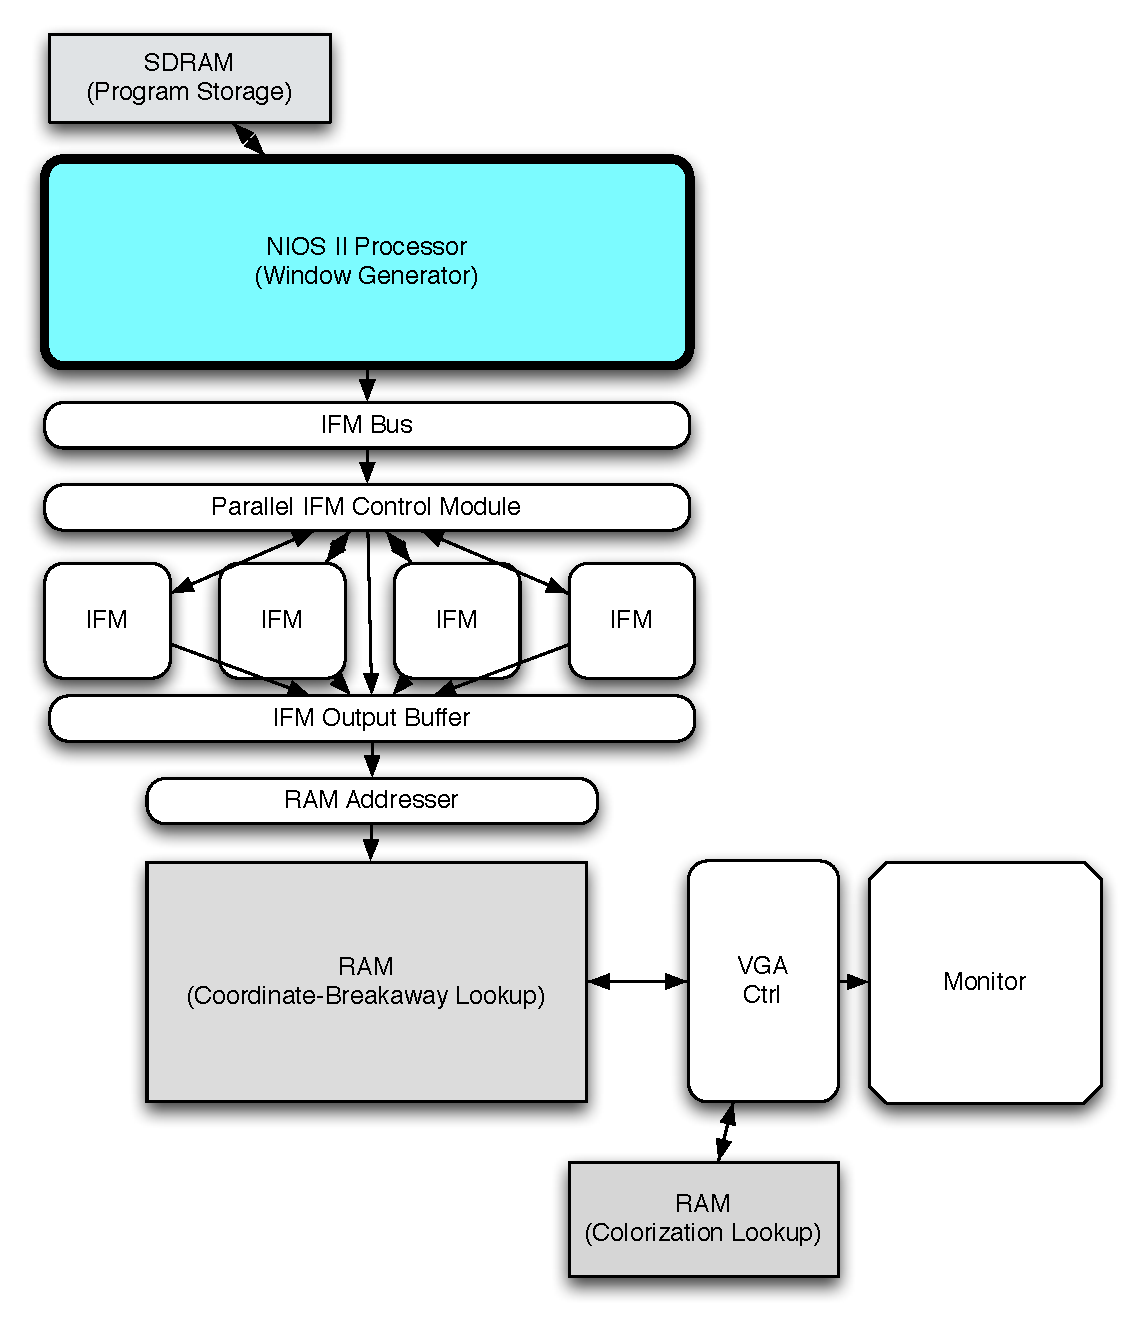
\includegraphics[width=\textwidth]{block_diagram.pdf}
  \caption{High-level Block Diagram}
\end{figure}
\newpage

% ------------------------------------------------------------
% now, we delve into the lower levels of the implementation
% ------------------------------------------------------------
\section{Critical Modules}

% ----------------------------------------
\subsection{Window Generator}

The window generator serves to kick off the calculation cascade,
calculating the position of each pixel in the complex plane and
writing both to active memory linked up to the input queue (described
below).

In more detail, the module loops through each pixel given the screen
resolution, and maps it according to the translation of the origin as
well as the scale of the complex plane with respect to the VGA
screen. Since we may yet implement the translation of the origin as a
parameter mutable by the user, this seperation of concerns makes
sense.

We switched this module from a hardware implementation to code sitting
on top of the \verb!Nios II! processor. The processor uses a
specialized procedure to generate the window tuples. The procedure
requires only four divisions and two modulo operations, which are
executed once at procedure start time. The remainder of the operations
are additions and comparisons.

\begin{lstlisting}[caption="Window Generation Procedure"]
int row, col;
   
//configure our window
int y_max = /*max y value in window*/
int x_max = /*max x value in window*/
int y_min = /*min y value in window */
int x_min = /*min x value in window */

//set our iteration params

//to compute a and b, we will iterate through each pixel of the screen
//adding win_dim/screen_dim to a sum that starts at win_dim_min

//we will also have "leap" iterations, which are iterations in which
//the sum must be incremented by 1 to keep it on track towards screen_dim

//amount to add each iteration   
int x_delt = (x_max - x_min)/VGA_WIDTH;
int y_delt = (y_max - y_min)/VGA_HEIGHT;

//leap total is the number of times we'll need to increment our sum by 1
int x_leap_total = (x_max - x_min)%VGA_WIDTH;
int y_leap_total = (y_max - y_min)%VGA_HEIGHT;

//leap count will keep track of how many times we incremented our count by this value
int x_leap_count = 0;
int y_leap_count = 0;

//leap interval is the number of cycles between leaps
int x_leap_interval = VGA_WIDTH/x_leap_total;
int y_leap_interval = VGA_HEIGHT/y_leap_total;

//time since last leap
int x_last_leap = 0;
int y_last_leap = 0;

long a = x_min;
long b = y_min;

//initialize a data value that will be written to the board

printf("here...\n");   
for(row = VGA_HEIGHT-1; row >= 0; row--)    //bottom to top so our min is in the bottom left corner
{

a = x_min;

for(col = 0; col < VGA_WIDTH; col++)    //left to right across the row
{
    //concatenate bit vector
    //printf("a:%x\n",a);
    //printf("b:%x\n",b);
    //printf("here %d\n", foo++);
    if(a < 0)
        a |= (1 << AB_SIGN_BIT);
    if(b < 0)
        b |= (1 << AB_SIGN_BIT);
                   
    //write to board
    //IOWR_32DIRECT(JULIA_CALC_BASE, 0, (0x3));
    //printf("writing...\n");
    IOWR_32DIRECT(JULIA_CALC_BASE, 0, ((a<<4)|0x0));
    IOWR_32DIRECT(JULIA_CALC_BASE, 0, ((b<<4)|0x1));
    IOWR_32DIRECT(JULIA_CALC_BASE, 0, ((((col<<X_SHIFT)|row)<<4)|0x2));
    IOWR_32DIRECT(JULIA_CALC_BASE, 0, (0x3));
   
    //printf("written\n");
    //printf("done\n");           
   
    //increment the imaginary value
    a+= x_delt;           
   
    //leap if necessary
    if(x_last_leap >= x_leap_interval && x_leap_count < x_leap_total)
    {
        a++;
        x_last_leap = 0;
        x_leap_count++;
    }
    else
        x_last_leap++;          
   
}

//increment the imaginary value
b += y_delt;

//leap if necessary
if(y_last_leap >= y_leap_interval && y_leap_count < y_leap_total)
{
    b++;
    y_last_leap = 0;
    y_leap_count++;
}
else
    y_last_leap++;

}
\end{lstlisting}

We have the Nios II configured to use the SDRAM as it's memory store,
since we use the, making the SRAM available for other uses.



% ----------------------------------------
\subsection{Iterative Function Module (IFM)}

Rendering Julia set fractals requires many iterations of relatively
simple computations in the complex plane. This sequence of
computations is independent for each point in the image, which is why
the calculation of fractal sets lends itself to parallel
computation. However, the very nature of the iterated fractal
calculation means that the run lengths of the individual calculations
are heterogenous, introducing synchronization issues.

With a pair of queues handling the heterogenity of the fractal
calculations, the IFM merely need calculate applications of the function:

\begin{equation}
f(z) = z^2 + c
\end{equation}

repeatedly, where $z,c \in \mathbb{C}$.

The complex nature of the calculations means that there need be 3
multiplications, not just 1, to find the next iteration of $z$.

Numbers are represented as two's-complement fixed-point binary
values. We restrict ourselves to 18 bits, as the onboard multipliers
are sized such. In order to accomodate the largest-magnitude value we
expect to come across during any iteration, we require 6 bits to the
left of the radix. Thus, our fixed-point values ahve 12 bits to the
right of the radix.

We count 127 iterations: after the 127th iteration, we consider the
originating point bounded.

We pass a pixel position and point on the complex plane to the IFM
through the queue. The complex plane position is meant to
facilitate the fractal calculation and the pixel position is meant for
display on the screen.



% ----------------------------------------
\subsection{Parallel IFM Control Module}

Documentation not complete.

\subsection{Coordinate-Breakaway Lookup Table}

We store the iteration counts in the on-chip RAM module, which offers
approximately 400 kilobytes of storage space.  We are using a $640
\times 480$ pixel display, and plan on storing 8 bits of breakaway
information. As such, we fill 307.2 kilobytes, or about 75\% of the
available RAM.

With a $640 \times 480$ screen size, rows nor columns automatically fit
nicely into the power of 2 sizes, and multiplication is
expensive. However, addressing the pixels column-first means that an
entire column fits in 240 16-bit words, and there is room to spare if
the row index is merely shifted 8 bits to the left, a fast operation.



% ----------------------------------------
\subsection{VGA Module}

A VGA controller is connected to the Coordinate-Breakaway lookup table
in order to display the generated Julia set. As the controller cycles
through output coordinates within the display area, it modifies the
read address signal for the lookup table. The data signal coming from
the RAM is thus the breakaway value associated with that coordinate.

This breakaway value is passed through a decoder known as the
Colorization Lookup Table and the resulting $(R, G, B)$ signal tuple
is sent to the VGA.



% ------------------------------------------------------------
\section{Parametrization Modules}

These modules can be used parameterize the output fractal

\begin{itemize}
\item PS/2 Keyboard input can be used to allow the user to specify
  fractal recomputation using a different set of parameters,
  permitting the modification of window ranges and Julia Set
  constants. Keyboard input would be facilitated through the Nios II
  processor and would require a reexecution of the Window Generator.
\item We could create a module for permuting the display colors given
  by the Colorization Lookup table using a periodic function, thus
  causing the colors to cycle. This module would allow us to modify
  the way the fractal looks without recomputing it.
\item Spectral analysis module takes audio input and uses it to
  influence the behavior of the Color Permutation module.
\end{itemize}


% ------------------------------------------------------------
% !!! UPDATE MILESTONES IF NECESSARY
\section{Updated Milestones}

\begin{itemize}
\item Milestone 1 (Mar 27): \\
  Develop a Window Generator and
  Parallelized IFM module that can communicate successfully.
\item Milestone 2 (Apr 10): \\
  Display the colorized (and static) Julia set through VGA.
\item Milestone 3 (Apr 24): \\ 
  Implement parameter mutation, with subsequent updates to the
  displayed Julia set.
\item Final Report and Presentation (May 10)
\end{itemize}

\end{document}
